\section{Třetí verze}
\label{M3-vyvoj}

\begin{wrapfigure}{R}{0.3\textwidth}
    \centering
    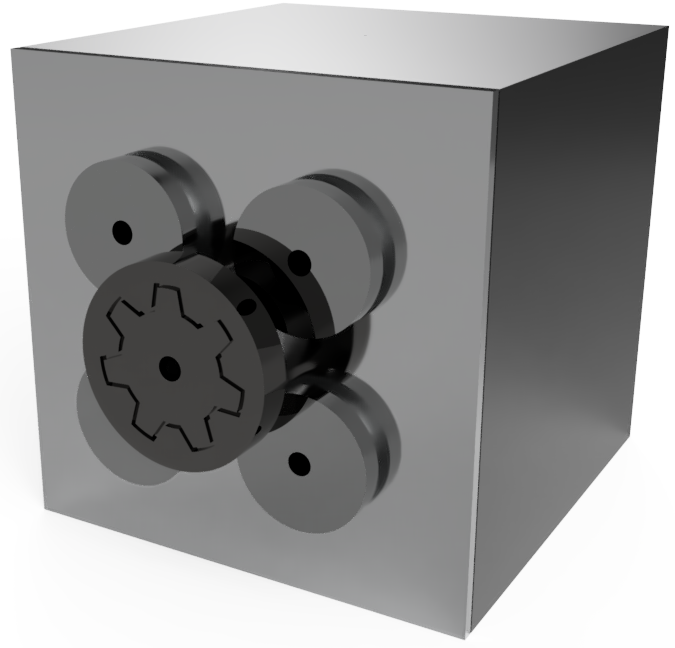
\includegraphics[width=0.3\textwidth]{kapitoly/obrazky/M3/predni_render.png}
    \caption{Render varianty M3}
    \label{fig:M3-miny-render}
\end{wrapfigure}

Dnešní mechanická varianta (M3) je téměř stejná jako druhá verze, rozdíl je jen v~uložení kol, které kolem hřídelů získalo distanční kroužky, které
zjednodušují lepení. 

Podrobnější popis mechanického trezoru M3 je v následující kapitole. 

\begin{figure}[h]
    \centering
    \vspace{40mm}
    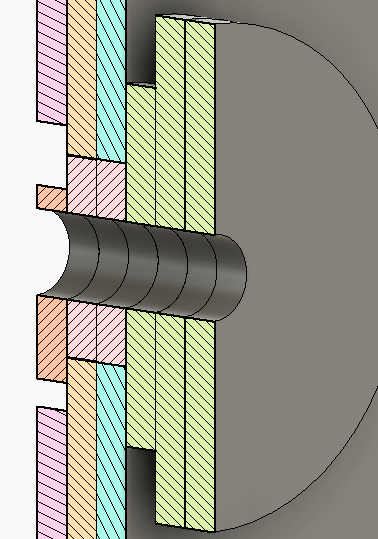
\includegraphics[width=0.4\textwidth]{kapitoly/obrazky/M3/rez.png}
    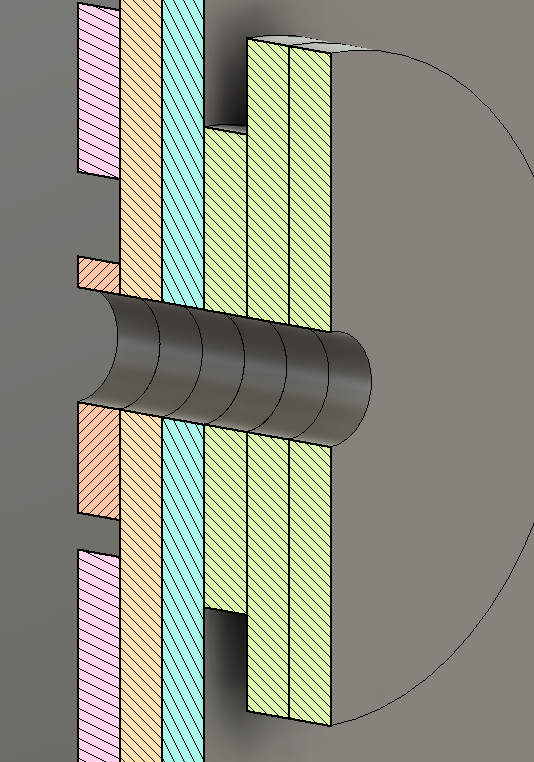
\includegraphics[width=0.4\textwidth]{kapitoly/obrazky/M2/rez.png}
    \caption{Řez kódovacím kolem trezoru M2 vpravo a řez kódovacím kolem trezoru M3 vlevo \centering}
    \label{fig:M3-rez-kolem}
\end{figure}

\newpage